\documentclass{beamer}

% Should be documentclass beamer

\mode<presentation>
{
%  \usetheme[hideothersubsections]{PaloAlto}
  \usetheme{metropolis}
  \setbeamercovered{transparent}
}

\usepackage{amsfonts}
\usepackage{amsmath}
\usepackage{amssymb}
\usepackage{color}
\usepackage{tikz}
\usepackage{pgfplots}
\usepackage{listings}
\usepackage{courier}
%\usepackage[utf8]{inputenc}
%\usepackage[russian]{babel}

\lstset{
  numbers=left,
  basicstyle=\ttfamily\footnotesize,
  numberstyle=\tiny\color{gray},
  stepnumber=1,
  numbersep=10pt,
}

\newcommand{\iu}{\ensuremath{\mathrm{i}}}
\newcommand{\bbR}{\mathbb{R}}
\newcommand{\bbC}{\mathbb{C}}
\newcommand{\calV}{\mathcal{V}}
\newcommand{\calW}{\mathcal{W}}
\newcommand{\macheps}{\epsilon_{\mathrm{mach}}}
\newcommand{\matlab}{\textsc{Matlab}}

\newcommand{\ddiag}{\operatorname{diag}}
\newcommand{\fl}{\operatorname{fl}}
\newcommand{\nnz}{\operatorname{nnz}}
\newcommand{\tr}{\operatorname{tr}}
\renewcommand{\vec}{\operatorname{vec}}

\newcommand{\vertiii}[1]{{\left\vert\kern-0.25ex\left\vert\kern-0.25ex\left\vert #1
    \right\vert\kern-0.25ex\right\vert\kern-0.25ex\right\vert}}
\newcommand{\ip}[2]{\langle #1, #2 \rangle}
\newcommand{\ipx}[2]{\left\langle #1, #2 \right\rangle}
\newcommand{\order}[1]{O( #1 )}

\newcommand{\kron}{\otimes}


\newcommand{\hdr}[2]{
  \title[CS 5220, Fall 2017]{CS 5220: #2}
  \author{David Bindel}
  \date{#1}
}


\hdr{2017-09-26}{Shared memory programming}

\begin{document}

\begin{frame}
  \titlepage
\end{frame}


\begin{frame}
  \frametitle{Message passing pain}

  Common message passing pattern
  \begin{itemize}
  \item Logical {\em global} structure
  \item {\em Local} representation per processor
  \item Local data may have redundancy
    \begin{itemize}
    \item Example: Data in ghost cells
    \item Example: Replicated book-keeping data ({\tt pidx} in our code)
    \end{itemize}
  \end{itemize}

  \vspace{5mm}
  Big pain point:
  \begin{itemize}
  \item Thinking about many partly-overlapping representations
  \item Maintaining consistent picture across processes
  \end{itemize}

  \vspace{5mm}
  Wouldn't it be nice to have just one representation?
\end{frame}

\begin{frame}
  \frametitle{Shared memory vs message passing}

  \begin{itemize}
  \item Implicit communication via memory vs explicit messages
  \item Still need separate global vs local picture?
    \begin{itemize}
    \item {\bf No:} One thread-safe data structure may be easier
    \item {\bf Yes:} More sharing can hurt performance
      \begin{itemize}
      \item Synchronization costs cycles even with no contention
      \item Contention for locks reduces parallelism
      \item Cache coherency can slow even non-contending access
      \end{itemize}
    \end{itemize}
  \item ``Easy'' approach: add multi-threading to serial code
  \item Better performance: design like a message-passing code
  \end{itemize}
  Let's dig a little deeper into the hardware side of this...
  
\end{frame}


\begin{frame}
  \frametitle{Memory model}

  \begin{itemize}
  \item Single processor: return last write
    \begin{itemize}
    \item What about DMA and memory-mapped I/O?
    \end{itemize}
  \item Simplest generalization: {\em sequential consistency} -- as if
    \begin{itemize}
    \item Each process runs in program order
    \item Instructions from different processes are interleaved
    \item Interleaved instructions ran on one processor
    \end{itemize}
  \end{itemize}
\end{frame}


\begin{frame}
  \frametitle{Sequential consistency}

  \begin{quote}
    A multiprocessor is sequentially consistent if the result
    of any execution is the same as if the operations of all the
    processors were executed in some sequential order, and the
    operations of each individual processor appear in this sequence
    in the order specified by its program. \\
    \hfill -- Lamport, 1979
  \end{quote}

\end{frame}


\begin{frame}[fragile]
  \frametitle{Example: Spin lock}

Initially, {\tt flag = 0} and {\tt sum = 0}

\vspace{5mm}
\hspace{0.04\textwidth}
\begin{minipage}{0.45\textwidth}
Processor 1:
\begin{verbatim}
sum += p1;
flag = 1;
\end{verbatim}
\end{minipage}
\begin{minipage}{0.45\textwidth}
Processor 2:
\begin{verbatim}
while (!flag);
sum += p2;
\end{verbatim}
\end{minipage}

\end{frame}


\begin{frame}[fragile]
  \frametitle{Example: Spin lock}

Initially, {\tt flag = 0} and {\tt sum = 0}

\vspace{5mm}
\hspace{0.04\textwidth}
\begin{minipage}{0.45\textwidth}
Processor 1:
\begin{verbatim}
sum += p1;
flag = 1;
\end{verbatim}
\end{minipage}
\begin{minipage}{0.45\textwidth}
Processor 2:
\begin{verbatim}
while (!flag);
sum += p2;
\end{verbatim}
\end{minipage}

\vspace{5mm}
Without sequential consistency support, what if
\begin{enumerate}
\item Processor 2 caches {\tt flag}?
\item Compiler optimizes away loop?
\item Compiler reorders assignments on P1?
\end{enumerate}
Starts to look restrictive!

\end{frame}


\begin{frame}
  \frametitle{Sequential consistency: the good, the bad, the ugly}
  
  Program behavior is ``intuitive'':
  \begin{itemize}
  \item Nobody sees garbage values
  \item Time always moves forward
  \end{itemize}
  One issue is {\em cache coherence}:
  \begin{itemize}
  \item Coherence: different copies, same value
  \item Requires (nontrivial) hardware support
  \end{itemize}
  Also an issue for optimizing compiler!

  \vspace{1cm}
  There are cheaper {\em relaxed} consistency models.
\end{frame}


\begin{frame}
  \frametitle{Snoopy bus protocol}

  % Need picture
  Basic idea:
  \begin{itemize}
  \item Broadcast operations on memory bus
  \item Cache controllers ``snoop'' on all bus transactions
    \begin{itemize}
    \item Memory writes induce serial order
    \item Act to enforce coherence (invalidate, update, etc)
    \end{itemize}
  \end{itemize}

  Problems:
  \begin{itemize}
  \item Bus bandwidth limits scaling
  \item Contending writes are slow
  \end{itemize}

  \vspace{5mm}
  There are other protocol options (e.g. directory-based). \\
  But usually give up on {\em full} sequential consistency.

\end{frame}


\begin{frame}
  \frametitle{Weakening sequential consistency}

  Try to reduce to the {\em true} cost of sharing
  \begin{itemize}
  \item {\tt volatile} tells compiler when to worry about sharing
  \item Memory fences tell when to force consistency
  \item Synchronization primitives (lock/unlock) include fences
  \end{itemize}
  
\end{frame}


\begin{frame}
  \frametitle{Sharing}
  
  True sharing:
  \begin{itemize}
  \item Frequent writes cause a bottleneck.
  \item Idea: make independent copies (if possible).
  \item Example problem: malloc/free data structure.
  \end{itemize}
  
  \vspace{5mm}
  False sharing:
  \begin{itemize}
  \item Distinct variables on same cache block
  \item Idea: make processor memory contiguous (if possible)
  \item Example problem: array of ints, one per processor
  \end{itemize}
\end{frame}


\begin{frame}
  \frametitle{Take-home message}

  \begin{itemize}
  \item Sequentially consistent shared memory is a useful idea...
    \begin{itemize}
    \item ``Natural'' analogue to serial case
    \item Architects work hard to support it
    \end{itemize}
  \item ... but implementation is costly!
    \begin{itemize}
    \item Makes life hard for optimizing compilers
    \item Coherence traffic slows things down
    \item Helps to limit sharing
    \end{itemize}
  \end{itemize}
  \vspace{1cm}
  Have to think about these things to get good performance.

\end{frame}


\begin{frame}
  \frametitle{Back to software...}
\end{frame}


\begin{frame}
  \frametitle{Reminder: Shared memory programming model}
  
  Program consists of {\em threads} of control.
  \begin{itemize}
  \item Can be created dynamically
  \item Each has private variables (e.g.~local)
  \item Each has shared variables (e.g.~heap)
  \item Communication through shared variables
  \item Coordinate by synchronizing on variables
  \item Examples: pthreads, OpenMP, Cilk, Java threads
  \end{itemize}

\end{frame}


\begin{frame}
  \frametitle{Wait, what's a thread?}

  Processes have {\em separate state}.  Threads share {\em some}:
  \begin{itemize}
  \item Instruction pointer (per thread)
  \item Register file (per thread)
  \item Call stack (per thread)
  \item Heap memory (shared)
  \end{itemize}

\end{frame}


\begin{frame}
  \frametitle{Mechanisms for thread birth/death}

  \begin{itemize}
  \item Statically allocate threads at start
  \item Fork/join (pthreads)
  \item Fork detached threads (pthreads)
  \item Cobegin/coend (OpenMP?)
    \begin{itemize}
    \item Like fork/join, but lexically scoped
    \end{itemize}
  \item Futures
    \begin{itemize}
    \item {\tt v = future(somefun(x))}
    \item Attempts to use {\tt v} wait on evaluation
    \end{itemize}
  \end{itemize}
\end{frame}


\begin{frame}
  \frametitle{Mechanisms for synchronization}

  \begin{itemize}
  \item Locks/mutexes (enforce mutual exclusion)
  \item Condition variables (notification)
  \item Monitors (like locks with lexical scoping)
  \item Barriers
  \item Atomic operations
  \end{itemize}
\end{frame}


\begin{frame}
  \frametitle{Getting more concrete...}
\end{frame}


\begin{frame}
  \frametitle{OpenMP: Open spec for MultiProcessing}

  \begin{itemize}
  \item Standard API for multi-threaded code
    \begin{itemize}
    \item Only a spec --- multiple implementations
    \item Lightweight syntax
    \item C or Fortran (with appropriate compiler support)
    \end{itemize}
  \item High level:
    \begin{itemize}
    \item Preprocessor/compiler directives (80\%)
    \item Library calls (19\%)
    \item Environment variables (1\%)
    \end{itemize}
  \item Basic syntax: {\tt \#omp {\it construct} [{\it clause} ...]}
    \begin{itemize}
    \item Usually affects structured block (one way in/out)
    \item OK to have {\tt exit()} in such a block
    \end{itemize}
  \end{itemize}
\end{frame}


\begin{frame}[fragile]
  \frametitle{A logistical note}

  A practical aside...
  \begin{itemize}
  \item Intel has OpenMP support by default
\begin{verbatim}
  icc -c -qopenmp foo.c
  icc -o -qopenmp mycode.x foo.o
\end{verbatim}
  \item GCC has OpenMP support by default (several years)
\begin{verbatim}
  gcc -c -fopenmp foo.c
  gcc -o -fopenmp mycode.x foo.o
\end{verbatim}
  \item LLVM has OpenMP support by default (more recent)
\begin{verbatim}
  clang -c -fopenmp foo.c
  clang -o -fopenmp mycode.x foo.o
\end{verbatim}
  \item Apple LLVM {\em does not} support OpenMP
    \begin{itemize}
    \item And {\tt gcc} on OS X now aliases {\tt clang}
    \item Can use Hombrew for alternate compiler
    \end{itemize}
  \end{itemize}
\end{frame}


\begin{frame}[fragile]
  \frametitle{Parallel ``hello world''}

\begin{lstlisting}
#include <stdio.h>
#include <omp.h>

int main()
{
    #pragma omp parallel
    printf("Hello world from %d\n", 
           omp_get_thread_num());

    return 0;
}
\end{lstlisting}
\end{frame}


\begin{frame}
  \frametitle{Shared and private}

  Annotations distinguish between different types of sharing:
  \begin{itemize}
  \item {\tt shared(x)} (default): One {\tt x} shared everywhere
  \item {\tt private(x)}: Thread gets own {\tt x} (indep.~of master)
  \item {\tt firstprivate(x)}: Each thread gets its own {\tt x},
    initialized by {\tt x} from before parallel region
  \item {\tt lastprivate(x)}: After the parallel region, private
    {\tt x} set to the value last left by one of the threads
  \item {\tt reduction(op:x)}: Does reduction on all thread {\tt x}
    on exit of parallel region
  \end{itemize}
\end{frame}


\begin{frame}
  \frametitle{Parallel regions}

  \begin{center}
  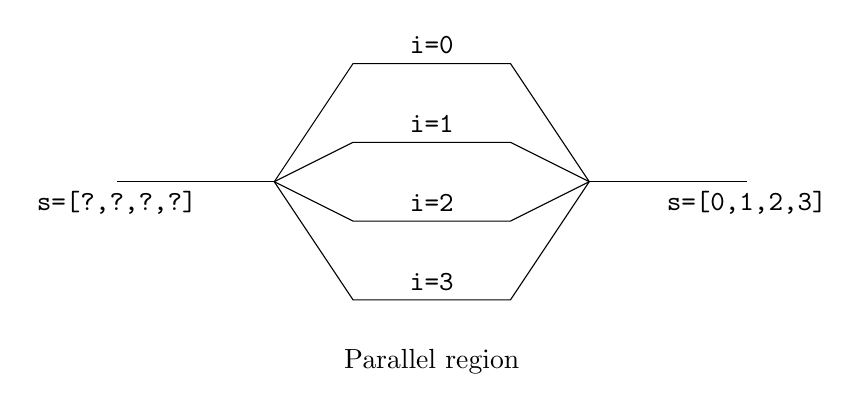
\begin{tikzpicture}
    \draw (-2,0) node[below] {\tt s=[?,?,?,?]} -- (0,0);
    \draw (0,0) -- (1, 1.5) -- (3, 1.5) node[midway,above] {\tt i=0} -- (4,0);
    \draw (0,0) -- (1, 0.5) -- (3, 0.5) node[midway,above] {\tt i=1} -- (4,0);
    \draw (0,0) -- (1,-0.5) -- (3,-0.5) node[midway,above] {\tt i=2} -- (4,0);
    \draw (0,0) -- (1,-1.5) -- (3,-1.5) node[midway,above] {\tt i=3} -- (4,0);
    \draw (4,0) -- (6,0) node[below] {\tt s=[0,1,2,3]};
    \node[below] at (2,-2) {Parallel region};
  \end{tikzpicture}
  \end{center}
  \begin{itemize}
  \item Basic model: fork-join 
  \item Each thread runs same code block
  \item Annotations distinguish shared ($s$) and private ($i$) data
  \item {\em Relaxed consistency} for shared data
  \end{itemize}

\end{frame}


\begin{frame}[fragile]
  \frametitle{Parallel regions}

  \begin{center}
  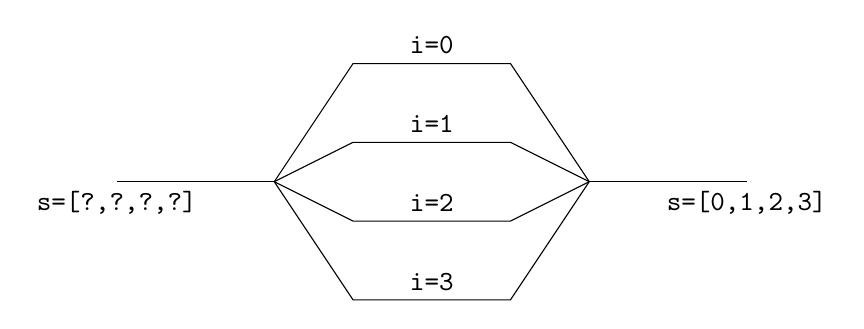
\begin{tikzpicture}
    \draw (-2,0) node[below] {\tt s=[?,?,?,?]} -- (0,0);
    \draw (0,0) -- (1, 1.5) -- (3, 1.5) node[midway,above] {\tt i=0} -- (4,0);
    \draw (0,0) -- (1, 0.5) -- (3, 0.5) node[midway,above] {\tt i=1} -- (4,0);
    \draw (0,0) -- (1,-0.5) -- (3,-0.5) node[midway,above] {\tt i=2} -- (4,0);
    \draw (0,0) -- (1,-1.5) -- (3,-1.5) node[midway,above] {\tt i=3} -- (4,0);
    \draw (4,0) -- (6,0) node[below] {\tt s=[0,1,2,3]};
  \end{tikzpicture}
  \end{center}
\begin{lstlisting}
double s[MAX_THREADS];
int i;
#pragma omp parallel shared(s) private(i)
{
  i = omp_get_thread_num();
  s[i] = i;
}
// Implicit barrier here
\end{lstlisting}
\end{frame}


\begin{frame}[fragile]
  \frametitle{Parallel regions}

  \begin{center}
  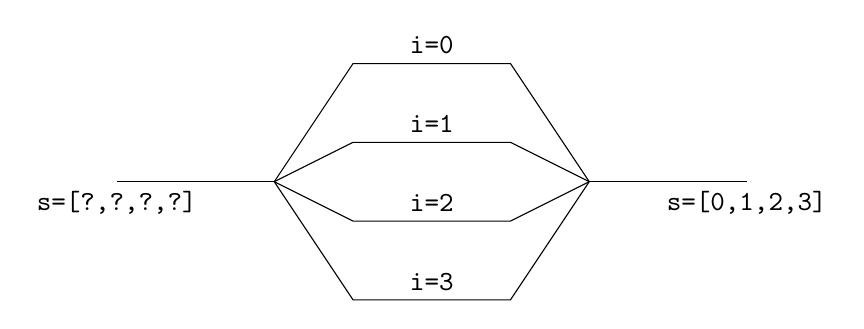
\begin{tikzpicture}
    \draw (-2,0) node[below] {\tt s=[?,?,?,?]} -- (0,0);
    \draw (0,0) -- (1, 1.5) -- (3, 1.5) node[midway,above] {\tt i=0} -- (4,0);
    \draw (0,0) -- (1, 0.5) -- (3, 0.5) node[midway,above] {\tt i=1} -- (4,0);
    \draw (0,0) -- (1,-0.5) -- (3,-0.5) node[midway,above] {\tt i=2} -- (4,0);
    \draw (0,0) -- (1,-1.5) -- (3,-1.5) node[midway,above] {\tt i=3} -- (4,0);
    \draw (4,0) -- (6,0) node[below] {\tt s=[0,1,2,3]};
  \end{tikzpicture}
  \end{center}
\begin{lstlisting}
double s[MAX_THREADS];  // default shared
#pragma omp parallel
{
  int i = omp_get_thread_num();  // local, so private
  s[i] = i;
}
// Implicit barrier here
\end{lstlisting}
\end{frame}


\begin{frame}
  \frametitle{Parallel regions}

  Several ways to control num threads
  \begin{itemize}
  \item Default: System chooses (= number processors?)
  \item Environment: {\tt export OMP\_NUM\_THREADS=4}
  \item Function call: {\tt omp\_set\_num\_threads(4)}
  \item Clause: {\tt \#pragma omp parallel num\_threads(4)}
  \end{itemize}
  Can also nest parallel regions.
\end{frame}


\begin{frame}[fragile]
  \frametitle{Parallel regions}

  What to do with parallel regions alone?  Maybe Monte Carlo:
  \begin{lstlisting}
    double result = 0;
    #pragma omp parallel reduction(+:result)
      result = run_mc(trials) / omp_get_num_threads();
    printf("Final result: %f\n", result);
  \end{lstlisting}
  Anything more interesting needs synchronization.
\end{frame}


\begin{frame}
  \frametitle{OpenMP synchronization}

  High-level synchronization:
  \begin{itemize}
  \item {\tt critical}: Critical sections
  \item {\tt atomic}: Atomic update
  \item {\tt barrier}: Barrier
  \item {\tt ordered}: Ordered access (later)
  \end{itemize}
  Low-level synchronization:
  \begin{itemize}
  \item {\tt flush}
  \item Locks (simple and nested
  \end{itemize}
  We will stay high-level.
  
\end{frame}

\begin{frame}
  \frametitle{Critical sections}

  \begin{center}
    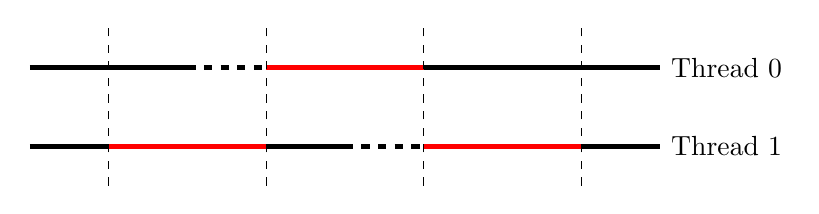
\begin{tikzpicture}
      \draw[ultra thick]         (0,0) -- (2,0);
      \draw[ultra thick, dashed] (2,0) -- (3,0);
      \draw[ultra thick, red]    (3,0) -- (5,0);
      \draw[ultra thick]         (5,0) -- (8,0) node[right] {Thread 0};

      \draw[ultra thick]         (0,-1) -- (1,-1);
      \draw[ultra thick, red]    (1,-1) -- (3,-1);
      \draw[ultra thick]         (3,-1) -- (4,-1);
      \draw[ultra thick, dashed] (4,-1) -- (5,-1);
      \draw[ultra thick, red]    (5,-1) -- (7,-1);
      \draw[ultra thick]         (7,-1) -- (8,-1) node[right] {Thread 1};

      \draw[dashed] (1, -1.5) -- (1, 0.5);
      \draw[dashed] (3, -1.5) -- (3, 0.5);
      \draw[dashed] (5, -1.5) -- (5, 0.5);
      \draw[dashed] (7, -1.5) -- (7, 0.5);
    \end{tikzpicture}
  \end{center}

  \begin{itemize}
  \item Automatically lock/unlock at ends of {\em critical section}
  \item Automatically memory flushes for consistency
  \item Locks are still there if you really need them...
  \end{itemize}
\end{frame}


\begin{frame}[fragile]
  \frametitle{Critical sections}

  \begin{center}
    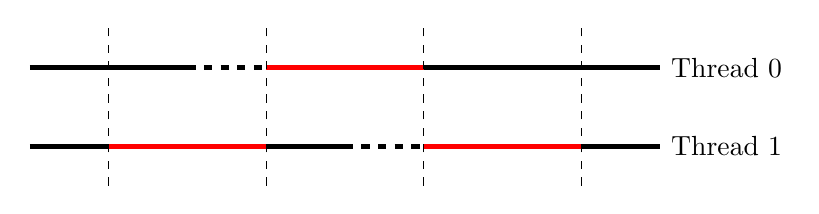
\begin{tikzpicture}
      \draw[ultra thick]         (0,0) -- (2,0);
      \draw[ultra thick, dashed] (2,0) -- (3,0);
      \draw[ultra thick, red]    (3,0) -- (5,0);
      \draw[ultra thick]         (5,0) -- (8,0) node[right] {Thread 0};

      \draw[ultra thick]         (0,-1) -- (1,-1);
      \draw[ultra thick, red]    (1,-1) -- (3,-1);
      \draw[ultra thick]         (3,-1) -- (4,-1);
      \draw[ultra thick, dashed] (4,-1) -- (5,-1);
      \draw[ultra thick, red]    (5,-1) -- (7,-1);
      \draw[ultra thick]         (7,-1) -- (8,-1) node[right] {Thread 1};

      \draw[dashed] (1, -1.5) -- (1, 0.5);
      \draw[dashed] (3, -1.5) -- (3, 0.5);
      \draw[dashed] (5, -1.5) -- (5, 0.5);
      \draw[dashed] (7, -1.5) -- (7, 0.5);
    \end{tikzpicture}
  \end{center}

\begin{lstlisting}
#pragma omp parallel {
  ...
  #pragma omp critical my_data_cs
  {
    ... modify data structure here ...
  }
}
\end{lstlisting}
\end{frame}


\begin{frame}[fragile]
  \frametitle{Atomic updates}

\begin{lstlisting}
#pragma omp parallel
{
  ...
  double my_piece = foo();
  #pragma omp atomic
  x += my_piece;
}
\end{lstlisting}
Only simple ops: increment/decrement or {\tt x += expr} and co

\end{frame}


\begin{frame}[fragile]
\frametitle{Barriers}

\begin{center}
%    \includegraphics[width=\textwidth]{barrier.pdf}
  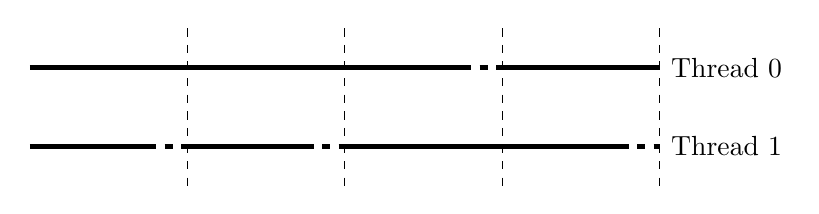
\begin{tikzpicture}
    \draw[ultra thick]         (0.0, 0) -- (5.5, 0);
    \draw[ultra thick, dashed] (5.5, 0) -- (6.0, 0);
    \draw[ultra thick]         (6.0, 0) -- (8.0, 0) node[right]
         {Thread 0};

    \draw[ultra thick]         (0.0,-1) -- (1.5,-1);
    \draw[ultra thick, dashed] (1.5,-1) -- (2.0,-1);
    \draw[ultra thick]         (2.0,-1) -- (3.5,-1);
    \draw[ultra thick, dashed] (3.5,-1) -- (4.0,-1);
    \draw[ultra thick]         (4.0,-1) -- (7.5,-1);
    \draw[ultra thick, dashed] (7.5,-1) -- (8.0,-1) node[right]
         {Thread 1};

    \draw[dashed] (2,0.5) -- (2,-1.5);
    \draw[dashed] (4,0.5) -- (4,-1.5);
    \draw[dashed] (6,0.5) -- (6,-1.5);
    \draw[dashed] (8,0.5) -- (8,-1.5);
  \end{tikzpicture}
\end{center}

\begin{lstlisting}
#pragma omp parallel
for (i = 0; i < nsteps; ++i) {
  do_stuff
  #pragma omp barrier
}
\end{lstlisting}
\end{frame}


\begin{frame}
  \frametitle{Is this all?}

  Next time:
  \begin{itemize}
  \item Parallel loop constructs
  \item Task-based parallelism (OpenMP 3.0+)
  \item Other parallel work divisions
  \end{itemize}
  But for now, let's do some examples!
\end{frame}

\end{document}
